\documentclass[a4paper]{article}

\usepackage[spanish]{babel}
\usepackage[utf8]{inputenc}
\usepackage{amsmath}
\usepackage{amssymb}
\usepackage{graphicx}
\usepackage[colorinlistoftodos]{todonotes}
\usepackage{multicol}
\setlength{\columnsep}{1cm}

\setlength{\parindent}{1em}
\setlength{\parskip}{1em}

\title{Demostración de la $\mathcal{NP}$-Completitud del problema del Circuito Hamiltoniano}

\author{Cristian Manuel Abrante Dorta, \\ Alberto Jesús González Álvarez, \\ Carlos Domínguez García, \\ Daute Rodríguez Rodríguez}

\date{9 de Enero de 2019}

\begin{document}
\maketitle

\newpage

\tableofcontents

\newpage

\section{Introducción}

\subsection{Descripción informal}

El problema \textit{Hamiltonian Circuit} consiste en determinar si dado un grafo, existe en él un \textit{Circuito Hamiltoniano}, esto es, un camino a través de los vértices del grafo de manera que se visite cada vértice una única vez y este comience y termine en el mismo vértice.

\subsection{Descripción formal}

Dado un grafo $G = (V, E)$:
\[V = \{v_{1}, v_{2}, \dots, v_{n}\}\quad|V| = n\]
\[E = \{\{u, v\}: u, v \in V\}\]

\textit{¿Contiene G un Camino Hamiltoniano?} Es decir, contiene \textit{G} una secuencia ordenada $<v_{1}, v_{2}, \dots, v_{n}>$ de tamaño $|V| = n$, tal que:

\[\{v_{n}, v_{1}\} \in E \land \{v_{i}, v_{i + 1}\} \in E \quad \forall i, 1 \leq i < n\]

\subsection{Motivación}

El estudio de este problema tiene diversas aplicaciones, en parte debido a su estrecha relación con el \textit{Traveling Salesman Problem}:
\begin{itemize}
    \item Problemas de rutas.
    \item Problemas de logística.
    \item Problemas de asignación de trabajos.
    \item Problemas de secuenciación de ADN.
\end{itemize}

\section{Demostración de $\mathcal{NP}$-Completitud}

\subsection{Introducción}

\begin{figure}[ht]
\centering
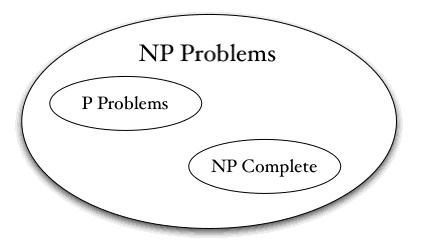
\includegraphics[width=0.5\textwidth]{images/p-np.jpg}
\caption{Diagrama $\mathcal{P-NP}$}
\end{figure}

Para demostrar que un problema $p$ pertenece a la clase de problemas $\mathcal{NP}$-Completo han de satisfacerse las dos condiciones siguientes:

\begin{enumerate}
    \item $p$ pertenece a la clase $\mathcal{NP}$, es decir, existe una \textbf{máquina de Turing no determinista} que resuelve el problema en tiempo polinomial.
    \[p \in \mathcal{NP}\]
    \item Existe una reducción polinomial de cada uno de los problemas de $\mathcal{NP}$ a $p$:
    \[\forall p' \in \mathcal{NP}, \quad p'\alpha\; p\]
\end{enumerate}

Típicamente, para demostrar la $\mathcal{NP}$-Completitud del problema \textit{Hamiltonian Circuit}, se lleva cabo una reducción polinomial del problema \textit{Vertex Cover}, probado como perteneciente a la clase de problemas $\mathcal{NP}$-Completo. Por ello, la siguiente sección del presente trabajo estará dedicada a definir la naturaleza del problema \textit{Vertex Cover}.

\begin{figure}[ht]
\centering
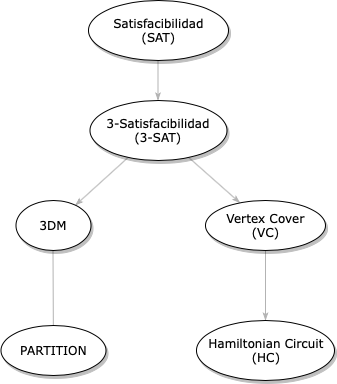
\includegraphics[width=0.5\textwidth]{images/NP-Completo-1.png}
\caption{Diagrama de problemas $\mathcal{NP}$-Completo}
\end{figure}

\subsection{Problema Vertex Cover}
Dado un grafo $G = (V, E)$ y un número entero $K \in \mathbb{N}\; /\; K < |V|$:
\[\exists V' \subseteq V, \quad |V'| \leq K : \{u, v\} \in E \to (u \in V') \lor (v \in V')\]
\textit{¿Existe un Vertex Cover de tamaño K?}. Es decir, ¿podemos encontrar un subconjunto $V'$ de vértices, de tal forma que cada arista es incidente en al menos uno de los vértices del conjunto?.

\subsection{Primera condición de $\mathcal{NP}$-Completitud}

\[HC \in \mathcal{NP}\]

Para demostrar que \textit{HC} pertenece al conjunto de problemas $\mathcal{NP}$-Completo basta con encontrar un algoritmo de \textbf{fuerza bruta}, que compruebe todas las permutaciones de vértices, lo cual presenta una complejidad temporal de:
\[\mathcal{O}(n!)\]

Dado un conjunto de vértices concreto, se puede comprobar si es un \textit{Camino Hamiltoniano} en \textbf{tiempo polinomial}.

\subsection{Segunda condición de $\mathcal{NP}$-Completitud}

\[\forall p' \in \mathcal{NP}, \quad p'\alpha\; p\]

Lo que es equivalente $VC \; \alpha \; HC$ puesto que $VC \in \mathcal{NP}-Completo$.

Partiendo del grador de entrada $G = (V, E)$ y el entero $K$, la demostración consiste en \textbf{construir en tiempo polinomial} un segundo grafo $G' = (V', E')$ de tal forma que, $G'$ contendrá un \textit{Circuito Hamiltoniano} sí y solo sí, existe un \textit{Vertex Cover} en $G$ de tamaño $K$ o inferior.

Cabe destacar que esta demostración se basa en la construcción de componentes.

\subsubsection{Selectores}

El primer conjunto de componentes será el de los \textbf{selectores}, el cual será un conjunto de vertices:
\[\{a_{1}, a_{2}, \dots, a_{k}\}\]
Utilizado para seleccionar los $K$ vértices del conjunto V de G.
\[a_{i}: 1 \leq i \leq K\]

\subsubsection{Componente cover-testing}

Construimos un componente \textbf{cover testing} por cada arista en $E$ ($\forall e \in E$). Con cada uno de estos componentes podremos garantizar que al menos uno de los vértices de esa arista está entre los $K$ vértices seleccionados.

Un componente cover-testing está formado por:
\begin{itemize}
    \item Un conjunto ($V'_e$) de doce vértices.
    \item Un conjunto ($E'_e$) de catorce aristas.
\end{itemize}

Construimos el cover testing de doce vértices definidos de la siguiente manera
\[V'_e = \{(u, e, i),(v,e,i) : i \le i \le 6\}\]

\begin{figure}[ht]
\centering
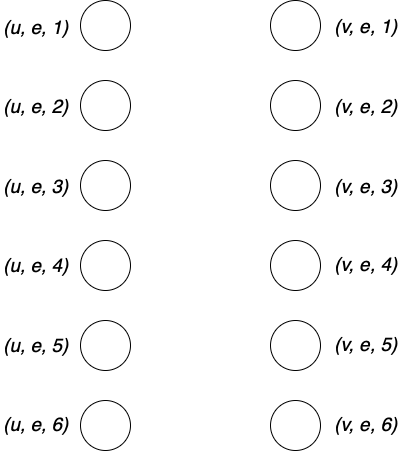
\includegraphics[scale=0.3]{images/cover-testing-1.png}
\end{figure}

A continuación definiremos las aristas que unirán los vértices. Estas aristas están definidas de la siguiente manera:
\begin{align*}
    E'_e = \{\{(u,e,i), (u,e, i+1)\},\{(v,e,i),(v,e,i+1)\} : i \le i < 6\} \\
    \cup \quad \{\{(u,e,3), (v,e,1)\},\{(v,e,3),(u,e,1)\}\} \\
    \cup \quad \{\{(u,e,6), (v,e,4)\},\{(v,e,6),(u,e,4)\}\}
\end{align*}

\begin{align*}
 a &= (a_1, a_2) \\
 b &= (b_1, b_2) \\
 &\phantom{b=\,} \vdots \\
 z &= (z_1, z_2)
\end{align*}
\begin{figure}[ht]
        \centering
        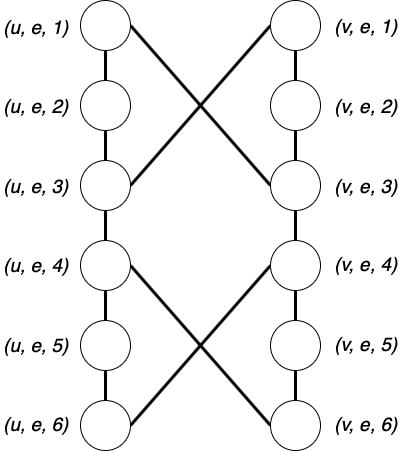
\includegraphics[scale=0.25]{images/cover-testing-2.png}
        \label{fig:my_label}
    \end{figure}
Los únicos vértices que aparecerán en alguna otra arista de G' serán:
\[(u,e,1) \quad (v,e,1) \quad (u,e,6) \quad (v,e,6)\]
De esta forma, se garantiza que cualquier \textbf{circuito hamiltoniano} de $G'$, recorrerá los vértices de $E'_e$, solo en una de estas tres formas:

\begin{figure*}[ht]
    \begin{multicols}{3}
    \begin{center}
            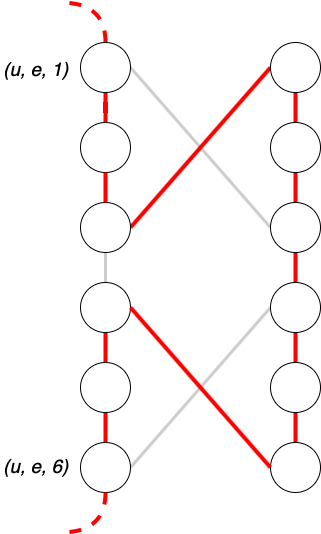
\includegraphics[scale=0.2]{images/cover-testing-3.png}
            \caption{$u$ está en el cubrimiento}
            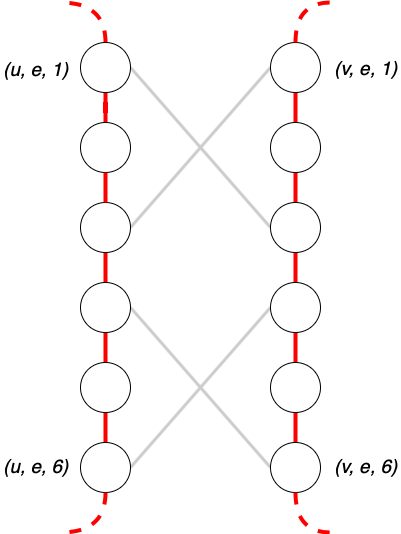
\includegraphics[scale=0.2]{images/cover-testing-4.png}
            \caption{$u$ y $v$ están en el cubrimiento}
            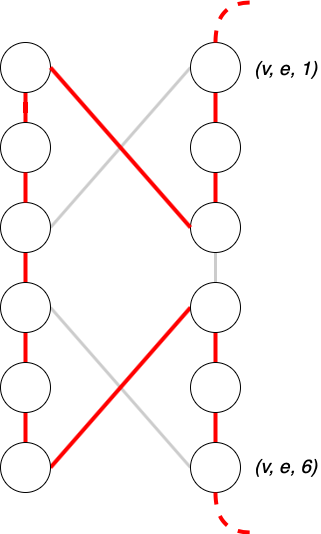
\includegraphics[scale=0.2]{images/cover-testing-5.png}
            \caption{$v$ está en el cubrimiento}
    \end{center}
    \end{multicols}
\end{figure*}

\subsubsection{Conexiones}

En primer lugar, se ordenan las aristas incidentes en cada vértice de manera arbitraria:
\[\forall v \in V, \quad <e_{v[1]}, e_{v[2]}, \cdots, e_{v[deg(v)]}>\]
Luego se construye el conjunto $E'_v$ de aristas que conectan \textbf{componentes cover-testing}:
\[E'_v = \{\{(v, e_{v[i]}, 6), (v, e_{v[i+1]},1)\} : 1 \le i < deg(v)\}\]
Finalmente, se conectan los finales de estos caminos con cada uno de \textbf{los selectores}:
\[E'' = \{\{a_i, (v,e_{v[1], 1})\},\{a_i, (v,e_{v[deg(v)]}, 6)\} : 1 \le i \le K, v \in V \}\]

\subsubsection{Generación del grafo}

Una vez hemos definido los componentes y conexiones, definimos $G'$ de la siguiente manera:
 \[G' = (V', E')\]
        \[V' = \{a_i : 1 \le i \le K\} \cup (\bigcup_{e \in E} V'_e)\]
        \[E' = (\bigcup_{e \in E} E'_e) \cup (\bigcup_{v \in V} E'_v) \cup E''\]

\subsubsection{Demostración de la segunda condición}
La demostración de II consiste en que si existe un VC de tamaño $K$ en $G$, entonces ha de existir un HC en $G'$. Por tanto, sea $V^* \subseteq V$ un Vertex Cover en $G$, de tamaño $K$: $V^* = \{v_1,v_2, \cdots, v_k \}$\\

Para cada \textbf{cover-testing}, se eligen los nodos dependiendo de la pertenencia al conjunto $V'$. Y a continuación se eligen las siguientes aristas:
\begin{itemize}
            \item $\{a_i, (v_i, e_{v_i[1]}, 1)\}, \quad 1 \le j \le K$
            \item $\{a_{i+1}, (v_1, e_{v_i[deg(v_i)]}, 6)\} \quad 1 \le i < K$
            \item $\{a_1, (v_K, e_{v_K[deg(v_K)]}, 6)\}$
\end{itemize}

Estas componentes formarán un \textbf{Circuito Hamiltoniano}.

\begin{thebibliography}{9}
\bibitem{GareyJohnson}
             Michael Garey, David S. Johnson.
            \newblock {\em Computers and Intractability: A Guide to the Theory of NP-Completeness}.
            \newblock W. H. Freeman and Company, 1979.
\bibitem{Jemand2000}
            Richard M. Karp.
            \newblock Reducibility Among Combinatorial Problems.
            \newblock {\em Complexity of Computer Computations}, pp:85-103, 1972.
\end{thebibliography}
\end{document}
